\documentclass[preprint,12pt,aps,pra,showkeys,amsmath,amssymb,superscriptaddress,floatfix]{revtex4-2}
\usepackage[T1]{fontenc}
\usepackage[utf8]{inputenc}
\usepackage{amsmath,amssymb,amsthm,mathtools,mathrsfs}
\usepackage{microtype,booktabs,enumitem}
\usepackage{xcolor,tikz,etoolbox}
\usepackage[skins,breakable]{tcolorbox}
\usepackage{needspace}
% Keep diagram geometry independent of REVTeX preprint body spacing.
\AtBeginEnvironment{tikzpicture}{\linespread{1}\selectfont}
\usetikzlibrary{arrows.meta,positioning,calc,fit,decorations.pathreplacing}
\usepackage{graphicx}
\usepackage{hyperref}

\definecolor{MMBlue}{RGB}{0,82,155}
\definecolor{MMOrange}{RGB}{200,80,0}
\tikzset{
 mmnode/.style={draw=MMBlue,rounded corners=2pt,fill=MMBlue!4,align=left,execute at begin node={\raggedright},text width=5cm,font=\fontsize{10}{12}\selectfont,inner sep=6pt},
 mmimport/.style={mmnode,draw=black!65,fill=black!4},
 mmcandidate/.style={mmnode,draw=MMOrange,dashed,fill=MMOrange!5},
 mmrejected/.style={mmnode,draw=black,densely dotted,fill=black!8},
 mmproof/.style={->,thick,MMBlue},
 mmflow/.style={->,semithick,black!70},
 mmrepair/.style={->,dashed,thick,MMOrange},
 mmcandidatearrow/.style={->,dashed,semithick,MMOrange},
 mmnote/.style={font=\scriptsize,fill=white,inner sep=2pt,align=center}}

\usepackage[section]{placeins}
\setlength{\emergencystretch}{3em}
\setlist{itemsep=3pt,topsep=4pt}
\newtheorem{theorem}{Theorem}[section]
\newtheorem{proposition}[theorem]{Proposition}
\newtheorem{lemma}[theorem]{Lemma}
\newtheorem{corollary}[theorem]{Corollary}
\theoremstyle{definition}
\newtheorem{definition}[theorem]{Definition}
\newtheorem{example}[theorem]{Example}
\theoremstyle{remark}
\newtheorem{remark}[theorem]{Remark}
% Avoid isolated statement headings and single-line paragraph fragments.
\BeforeBeginEnvironment{theorem}{\Needspace{6\baselineskip}}
\BeforeBeginEnvironment{definition}{\Needspace{5\baselineskip}}
\BeforeBeginEnvironment{proposition}{\Needspace{5\baselineskip}}
\BeforeBeginEnvironment{lemma}{\Needspace{5\baselineskip}}
\BeforeBeginEnvironment{corollary}{\Needspace{5\baselineskip}}
\clubpenalty=5000
\widowpenalty=5000
\newcommand{\R}{\mathbb R}\newcommand{\Z}{\mathbb Z}\newcommand{\N}{\mathbb N}
\newcommand{\Pa}{\operatorname{Pa}}\newcommand{\Desc}{\operatorname{Desc}}
\newcommand{\cl}{\operatorname{cl}}\newcommand{\cost}{\operatorname{cost}}
\newcommand{\status}{\operatorname{status}}
% Faculty cards: a visual rail groups the five faculties within one agent.
% The rail has no arrowhead and does not represent a proof dependency.
\newcommand{\mmfacultybadge}[1]{%
 \node[circle,draw=MMBlue,line width=1pt,fill=white,
 minimum size=7mm,inner sep=0pt,font=\sffamily\small\bfseries,text=MMBlue]
 at ([xshift=15pt,yshift=-15pt]frame.north west) {#1};}
\newcommand{\mmfacultyrail}{%
 \draw[MMBlue!80,line width=1pt]
 ([xshift=15pt,yshift=2pt]frame.north west)--
 ([xshift=15pt,yshift=-2pt]frame.south west);}
\newtcolorbox{mmfacultybox}[2]{enhanced,breakable,
 colback=MMBlue!4,colframe=MMBlue!4,boxrule=0pt,arc=3pt,
 left=39pt,right=9pt,top=4pt,bottom=4pt,
 before skip=2pt,after skip=2pt,
 fontupper=\small\linespread{1.1}\selectfont,
 overlay unbroken={\mmfacultyrail\mmfacultybadge{#1}},
 overlay first={\mmfacultyrail\mmfacultybadge{#1}},
 overlay middle={\mmfacultyrail},overlay last={\mmfacultyrail}}
\newcommand{\mmfaculty}[3]{%
 \begin{mmfacultybox}{#1}{#2}
 {\sffamily\bfseries\color{MMBlue}#2}\par\smallskip #3
 \end{mmfacultybox}}
\newcommand{\agent}[9]{%
 \Needspace{8\baselineskip}
 \subsubsection{#1}
 \noindent\textbf{Object.} #2\par
 \noindent\textbf{Role.} #3\par\smallskip
 \mmfaculty{E}{Ego}{#4}
 \mmfaculty{M}{Memory}{#5}
 \mmfaculty{I}{Intellect}{#6}
 \mmfaculty{S}{Sense}{#7}
 \mmfaculty{A}{Action}{#8}
 \smallskip\noindent #9\par}

\usepackage{longtable,array,calc}
\providecommand{\tightlist}{\setlength{\itemsep}{2pt}\setlength{\parskip}{0pt}}
\makeatletter
\def\frontmatter@abstract@produce{\par\addvspace{\frontmatter@preabstractspace}%
\begingroup\prep@absbox\unvbox\absbox\post@absbox\endgroup
\addvspace{\frontmatter@postabstractspace}}
\makeatother
\newcommand{\field}[2]{\par\smallskip\noindent\textbf{#1.} #2\par}
\setlength{\emergencystretch}{5em}
\AtBeginEnvironment{verbatim}{\small\linespread{1.0}\selectfont}


\hypersetup{colorlinks=true,linkcolor=MMBlue,urlcolor=MMBlue,pdfauthor={Dibakar Sigdel}}

\begin{document}

\title{Uniform Boundedness Principle\\[4pt]\large An End-to-End Meta-Math Walkthrough}

\author{Dibakar Sigdel}

\affiliation{Mindverse Computing LLC, Lynnwood, WA 98087, USA}

\date{October 2026}

\begin{abstract}

Convert bounds depending on the point into one common bound on a ball,
then subtract its center and rescale. The report presents the target
theorem, declared imports, a dependency graph, five-faculty node
contracts, a continuous proof, a worked example, and a hypothesis-repair
audit. It is an authored mathematical exposition, not a deployed-agent
transcript or a formal proof-assistant certificate.

\end{abstract}\maketitle\linespread{1.12}\selectfont

\noindent\textbf{FA-04 / Functional Analysis and Measure Theory / Report v1}

\section{Target and import contract}

\begin{theorem}

Let \(X\) be a Banach space, \(Y\) a normed space, and \(\mathcal T\) a
family of bounded linear maps \(X\to Y\). If for every \(x\in X\) the
number \(\sup_{T\in\mathcal T}\|Tx\|\) is finite, prove
\(\sup_{T\in\mathcal T}\|T\|<\infty\). The family need not be countable,
and \(Y\) need not be complete.

\end{theorem}

\subsection{Foundations and permitted imports}

Import the Baire category theorem: a nonempty complete metric space
cannot be a countable union of closed sets with empty interior. Use
continuity of bounded operators, the triangle inequality, and the
operator norm. The empty family satisfies the boundedness conclusion
vacuously; treat the nonempty case below.

\clearpage\section{Node interaction workflow}

\begin{center}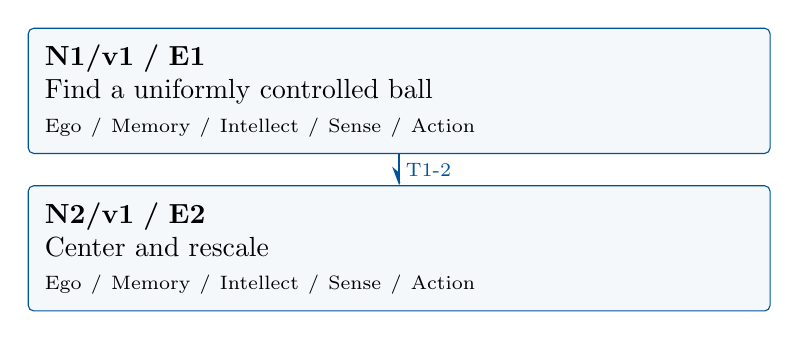
\begin{tikzpicture}[>=Stealth,x=1cm,y=1cm]

\node[mmnode,text width=9cm,minimum height=1.25cm] (N1) at (0,0.0) {\textbf{N1/v1 / E1}\\Find a uniformly controlled ball\\{\scriptsize Ego / Memory / Intellect / Sense / Action}};

\node[mmnode,text width=9cm,minimum height=1.25cm] (N2) at (0,-2.0) {\textbf{N2/v1 / E2}\\Center and rescale\\{\scriptsize Ego / Memory / Intellect / Sense / Action}};

\draw[mmproof] (N1.south) -- node[mmnote,right] {T1-2} (N2.north);

\end{tikzpicture}\end{center}

Each box is one mathematical agent containing all five faculties. Blue
arrows carry the versioned exports listed below. The layout gives a
reading order; only drawn arrows assert dependencies. Diagnostic repair
is separate from the proof DAG.

\subsection{Versioned evidence-transfer ledger}

\begingroup\small\linespread{1.05}\selectfont

\Needspace{5\baselineskip}\field{T1-2: N1/E1/v1 to N2}{There are \(N\), \(x_0\), and \(r>0\) with \(B(x_0,r)\subset F_N\).}

\field{Receiving activity}{N2.1}

\field{Compatibility}{E1/v1 and linearity of every \(T\). Check: The ball is not necessarily
centered at zero, so its center must be subtracted before scaling.}

\endgroup

\clearpage\section{Agent roles and five-faculty activities}\begingroup\small\linespread{1.05}\selectfont\setlist{itemsep=1pt,topsep=2pt}

\subsection{N1/v1: Find a uniformly controlled ball}

\field{Object and role}{Apply Baire to the countable collection of level sets, even when the
operator family is uncountable. \textbf{Local obligation:} There are
\(N\), \(x_0\), and \(r>0\) with \(B(x_0,r)\subset F_N\).}

\field{Inputs}{\(F_n=\{x:\sup_{T\in\mathcal T}\|Tx\|\le n\}\) for integers \(n\ge1\).}

\mmfaculty{E}{Ego}{Publish E1/v1 only after establishing this obligation: There are \(N\),
\(x_0\), and \(r>0\) with \(B(x_0,r)\subset F_N\).}

\mmfaculty{M}{Memory}{\(F_n=\{x:\sup_{T\in\mathcal T}\|Tx\|\le n\}\) for integers \(n\ge1\).
Retain the stated assumptions and import versions.}

\mmfaculty{I}{Intellect}{Apply Baire to the countable collection of level sets, even when the
operator family is uncountable.}

\mmfaculty{S}{Sense}{Each \(F_n\) is an arbitrary intersection of closed inverse images;
countability is needed for the cover by \(F_n\), not for \(\mathcal T\).}

\mmfaculty{A}{Action}{Carry out activities N1.1--N1.2 below, retaining each calculation and
construction as evidence.}

\smallskip\noindent\textbf{Numbered mathematical activities}

\begin{enumerate}[label=N1.\arabic*,leftmargin=3.4em]

\item For each \(T\), the set \(\{x:\|Tx\|\le n\}\) is closed by continuity,
so their intersection \(F_n\) is closed. Pointwise boundedness says
\(X=\bigcup_{n\ge1}F_n\).

\item The Banach space \(X\) is a nonempty complete metric space. Baire
therefore gives an \(F_N\) with nonempty interior, which contains some
open ball \(B(x_0,r)\). In particular \(x_0\in F_N\).

\end{enumerate}

\field{Export E1/v1}{There are \(N\), \(x_0\), and \(r>0\) with \(B(x_0,r)\subset F_N\).}

\field{Acceptance gate}{Each \(F_n\) is an arbitrary intersection of closed inverse images;
countability is needed for the cover by \(F_n\), not for \(\mathcal T\).}

\field{Targeted repair}{If Baire is applied to the operator index set, rebuild the countable
level-set cover of the complete space \(X\). Withhold this export and
recheck its descendants after a versioned correction.}

\clearpage

\subsection{N2/v1: Center and rescale}

\field{Object and role}{Use a difference of two points in the controlled ball to bound the unit
ball. \textbf{Local obligation:} For every \(T\in\mathcal T\),
\(\|T\|\le4N/r\).}

\field{Inputs}{E1/v1 and linearity of every \(T\). Incoming proof exports: E1/v1 at
N2.1.}

\mmfaculty{E}{Ego}{Publish E2/v1 only after establishing this obligation: For every
\(T\in\mathcal T\), \(\|T\|\le4N/r\).}

\mmfaculty{M}{Memory}{E1/v1 and linearity of every \(T\). Incoming proof exports: E1/v1 at
N2.1. Retain the stated assumptions and import versions.}

\mmfaculty{I}{Intellect}{Use a difference of two points in the controlled ball to bound the unit
ball.}

\mmfaculty{S}{Sense}{The ball is not necessarily centered at zero, so its center must be
subtracted before scaling.}

\mmfaculty{A}{Action}{Carry out activities N2.1--N2.2 below, retaining each calculation and
construction as evidence.}

\smallskip\noindent\textbf{Numbered mathematical activities}

\begin{enumerate}[label=N2.\arabic*,leftmargin=3.4em]

\item For \(\|h\|<r\), both \(x_0+h\) and \(x_0\) belong to \(F_N\), so
\(\|Th\|\le\|T(x_0+h)\|+\|Tx_0\|\le2N\) for every \(T\).

\item For \(\|u\|\le1\), choose \(h=(r/2)u\). Then
\(\|Tu\|=(2/r)\|Th\|\le4N/r\). Taking the supremum over the unit ball
and then the family proves the theorem. Completeness of \(Y\) was never
used.

\end{enumerate}

\field{Export E2/v1}{For every \(T\in\mathcal T\), \(\|T\|\le4N/r\).}

\field{Acceptance gate}{The ball is not necessarily centered at zero, so its center must be
subtracted before scaling.}

\field{Targeted repair}{If a candidate rescales \(x_0+h\) directly, replace it by the difference
\(h\) first; retain the factor two from the triangle inequality.
Withhold this export and recheck its descendants after a versioned
correction.}

\endgroup\clearpage\section{Continuous mathematical proof}\label{sec:proof}

\subsection{N1 --- Find a uniformly controlled
ball}\label{n1-find-a-uniformly-controlled-ball}

\begin{enumerate}
\def\labelenumi{\arabic{enumi}.}
\item
  \textbf{N1.1.} For each \(T\), the set \(\{x:\|Tx\|\le n\}\) is closed
  by continuity, so their intersection \(F_n\) is closed. Pointwise
  boundedness says \(X=\bigcup_{n\ge1}F_n\).
\item
  \textbf{N1.2.} The Banach space \(X\) is a nonempty complete metric
  space. Baire therefore gives an \(F_N\) with nonempty interior, which
  contains some open ball \(B(x_0,r)\). In particular \(x_0\in F_N\).
\end{enumerate}

\subsection{N2 --- Center and rescale}\label{n2-center-and-rescale}

\begin{enumerate}
\def\labelenumi{\arabic{enumi}.}
\item
  \textbf{N2.1.} For \(\|h\|<r\), both \(x_0+h\) and \(x_0\) belong to
  \(F_N\), so \(\|Th\|\le\|T(x_0+h)\|+\|Tx_0\|\le2N\) for every \(T\).
\item
  \textbf{N2.2.} For \(\|u\|\le1\), choose \(h=(r/2)u\). Then
  \(\|Tu\|=(2/r)\|Th\|\le4N/r\). Taking the supremum over the unit ball
  and then the family proves the theorem. Completeness of \(Y\) was
  never used.
\end{enumerate}

\hfill$\square$

\section{Worked orchestration}

On \(\ell^2\), take \(T_nx=x_n\). For each \(x\),
\(\sup_n|x_n|\le\|x\|_2\). Testing the standard basis gives
\(\|T_n\|=1\), so the pointwise and uniform bounds agree. The theorem
also applies when a direct formula for the common norm bound is
unavailable.

\subsection{Boundary and hypothesis audit}

On the incomplete normed space \(c_{00}\) with the sup norm, set
\(T_nx=n x_n\). Each \(T_n\) is bounded with norm \(n\). For each
finitely supported \(x\), only finitely many \(T_nx\) are nonzero, so
pointwise boundedness holds while uniform boundedness fails.

\section{Illustrative failure and repair}

The following is an authored diagnostic scenario. Changed assumptions
define a new contract; they do not retroactively prove the original
statement.

\subsection{Rejected argument, diagnosis, and correction}
\textbf{Rejected generalization (N1.2):} the theorem works for every
normed domain. \textbf{Sense:} \(c_{00}\) and \(T_nx=nx_n\) refute it.
\textbf{Diagnosis:} the Baire import requires completeness.
\textbf{Repair:} retain the original Banach-domain contract and apply
Baire exactly there; extending the target to arbitrary normed spaces
would require new assumptions. N2 may consume only the ball export
proved under completeness.

\subsection{Publication and reuse}
The corrected export retains its explicit assumptions. A hypothetical
revision receives a new version, and each consuming activity is
rechecked; this scenario is not a recorded runtime event. \textbf{Next
direction:} Combine this with pointwise convergence of bounded operators
to control their norms; convergence in operator norm still requires
additional hypotheses.

\par\medskip\begingroup\small\linespread{1.0}\selectfont\noindent\textbf{Provenance.} This authored proof is complete relative to its declared imports. Reuse
each export with its assumptions, proof, and version. The original
Markdown remains available for comparison.
\par\endgroup

\par\smallskip\begingroup\small\linespread{1.0}\selectfont\noindent\textbf{Further reading.} \href{https://ocw.mit.edu/courses/18-102-introduction-to-functional-analysis-spring-2021/resources/lecture-notes/}{MIT
OpenCourseWare, Introduction to Functional Analysis: lecture notes}. See
the lectures on integration, Hilbert spaces, Baire category, and
Hahn--Banach.\par\endgroup

\end{document}
